\subsubsection{HOMME Performance Results}\label{sec:homme-results}

We evaluate the impact of the threading changes described in Section \ref{sec:homme-alg} using two different configuration of the HOMME dynamical core.  The {\em perfTest} configuration uses 26 vertical levels (plev=26), and 25 tracers (qsize=25) and is similar to how the default configuration of CAM-SE.  The {\em perfTestWACCM} uses 70 vertical levels (plev=70) and 135 tracers (qsize=135) and is comparable to the default configuration used by the Whole Atmosphere Community Climate Model (WACCM) \cite{waccm}.  HOMME uses a cubed-sphere computational grid, and horizontal resolution is indicated by the number of spectral elements on a side of a cube (ne). CAM-SE is typically run in production at ne=30 which corresponds to grid points approximately every 100 km.  High resolution simulations with grid points approximately every 25 km (ne=120) typically require very large core counts for an extended periods of time.   For example ASD simulation \cite{asd} executed CAM-SE at 25 km resolution on 21,600 cores of Yellowstone in 20?? for ?4? months.

The performance of HOMME is strongly influenced by the number of spectral elements allocated to each hardware core.  The total number of spectral elements is calculated by the formula total\_elm = 6 * ne  * ne.  For the ne=120 ASD simulation a total of 86,400 spectral elements were used resulting in the assignment of 4 elements per core. For the purposes of our evaluations, several different horizontal resolution configurations are used, (ne=4, 8, and 30). The ne=4 resolution has a total of 96 total spectral elements, while the ne=8 and ne=30 have 384, and 5400.  We use the ne=4 and ne=8 configurations to measure the impact of our modifications on either a single node or small number of nodes.  The ne=30 configuration is to measure the impact of our modifications at much larger node counts.  

%The ne=30 configuration, which represents the current production resolution, has grid points approximately every 100 km.  The ne=4 and ne=8 configurations are typically not run in production, but are useful for evaluating performance of HOMME on either a single or small number of nodes.  While there have been several high-resolution simulations that utilize CAM-SE running at ne=120 (25 km) resolution \cite{asd,others}, these simulations require a long time to complete and utilize very large core counts.  For example ASD simulation executed CAM-SE at 25 km resolution on 21,600 cores of Yellowstone in 20?? for ?4? months.   

%Each spectral element consists of a [4x4] patch of grid points. 
% The Both configurations used [4x4] tensor product quadrature points within each element.  
%The experiments used for the performance studies were: perTestWACCM and perfTest with a baroclinic instability test case. These configurations were chosen as they represents the 'workhorse' for future experiments in the National Center for Atmospheric Research?s Community Climate System Model. Both experiments used NE=8 which represents a XX km horizontal resolution at the equator. The dynamics time-step for both cases was 480 seconds. For perTestWACCM there were 70 vertical levels with 135 tracers and for perfTest 25 vertical levels with 25 tracers. Both experiments used [4x4] tensor product quadrature points within each element. 

The execution time seconds/model day and the computational cost for both the original and optimized code is provided for the ne=4 configuration on Yellowstone is provided in Figure \ref{fig:homme-ys-ne4}.  Note that both the number of nodes used and the number of elements per hardware core is provided on the bottom and top x-axis on Figure \ref{fig:homme-ys-ne4}.  The left y-axis corresponds to the execution time in seconds per model day, while the right y-axis corresponds to the computational cost.  The lines in Figure \ref{fig:homme-ys-ne4}, which are solid and dashed with diamond data points that correspond to the execution time clearly illustrate the reduction in execution time.  Figure \ref{fig:homme-ys-ne4} clearly illustrates that non only does the optimized code reduce the execution time, but it also allowed HOMME to scale to larger core counts.  In particular, while HOMME was previously limited to a single element per hardware core, It is now possible to obtain speedup for this configuration out to $1/4$ element per hardware core.  The plain dotted line and dotted line with diamond data points indicate the computational cost relative to the original code on a single node.  These cost lines allow for an easy comparison of the impact that these optimizations may have on how HOMME is used.  While the optimized version of HOMME will certainly reduce the cost of simulations on a fixed number of cores, it also introduces the possibility to use more hardware for a fixed computational cost.  For example if we draw a horizontal line from the host to run HOMME using 6 elements per hardware core from the original code (plain dotted line) to the optimized code (dotted line with diamonds) it is apparent that is is now possible to increase the amount of hardware used from 1 node to 3 nodes without any increase in the computational cost.  The ability to efficiently utilize more hardware without increasing computational cost is a important advance for the optimized code.  

%If we draw a horizontal line from the cost to perform HOMME using 6 element per hardware core, 

 %If we draw a horizontal line from the cost to perform the CESM1 version of the SE dynamical core in the CAM-like configuration (left figure) using 3 elements per hardware core, it is apparent that we can utilize ~3 times the amount of hardware cores with only a very modest increase in computational cost using the new SE dynamical core.  Specifically, instead of using 3 elements per hardware core we can scale to 1 element per hardware core.  A similar analysis for WACCM-like configuration reveals that instead of being limited to 3 elements per hardware core, we will be able to scale to ¼ element per hardware core, enabling the use of 12 times the number of hardware cores. 

configuration has a total of 96 spectral elements, while our ¼-degree grid has a total of 86,400 spectral elements.  For our 2048-node production runs, we use a total of 64 execution threads per node which results in 2 or 3 spectral elements allocated to each 32K hardware core.  The left panel in Figure 5, which has an x-axis that varies from 6 to ¼ spectral element per hardware core, is a configuration of the SE dynamical core that has 26 vertical levels and 25 tracers and is similar to a standard CAM configuration.  We refer to this configuration of the SE dynamical core as CAM-like.  The right panel in Figure 5, in which the x-axis varies from 6 to 1/8 spectral elements per hardware core, is a configuration of the SE dynamical core that has 70 vertical levels and 135 tracers and is similar to a standard configuration of the Whole Atmosphere Community Climate Model (WACCM).  This particular configuration of the SE dynamical core we refer to as WACCM-like. 

%The simulations proposed here are not stated to use WACCM; however, one reason is that WACCM has been computationally expensive. With the performance enhancements described below, it may make it feasible for the future simulations with CESM2 to run with the WACCM atmosphere. Additionally, using WACCM or not, these enhancements are indicative of improvements that would occur when running the model with additional tracers or vertical levels (in either the atmosphere or ocean), which may be desirable as we become interested in higher resolution and additional output variables.


\begin{figure}[]
 \begin{center}
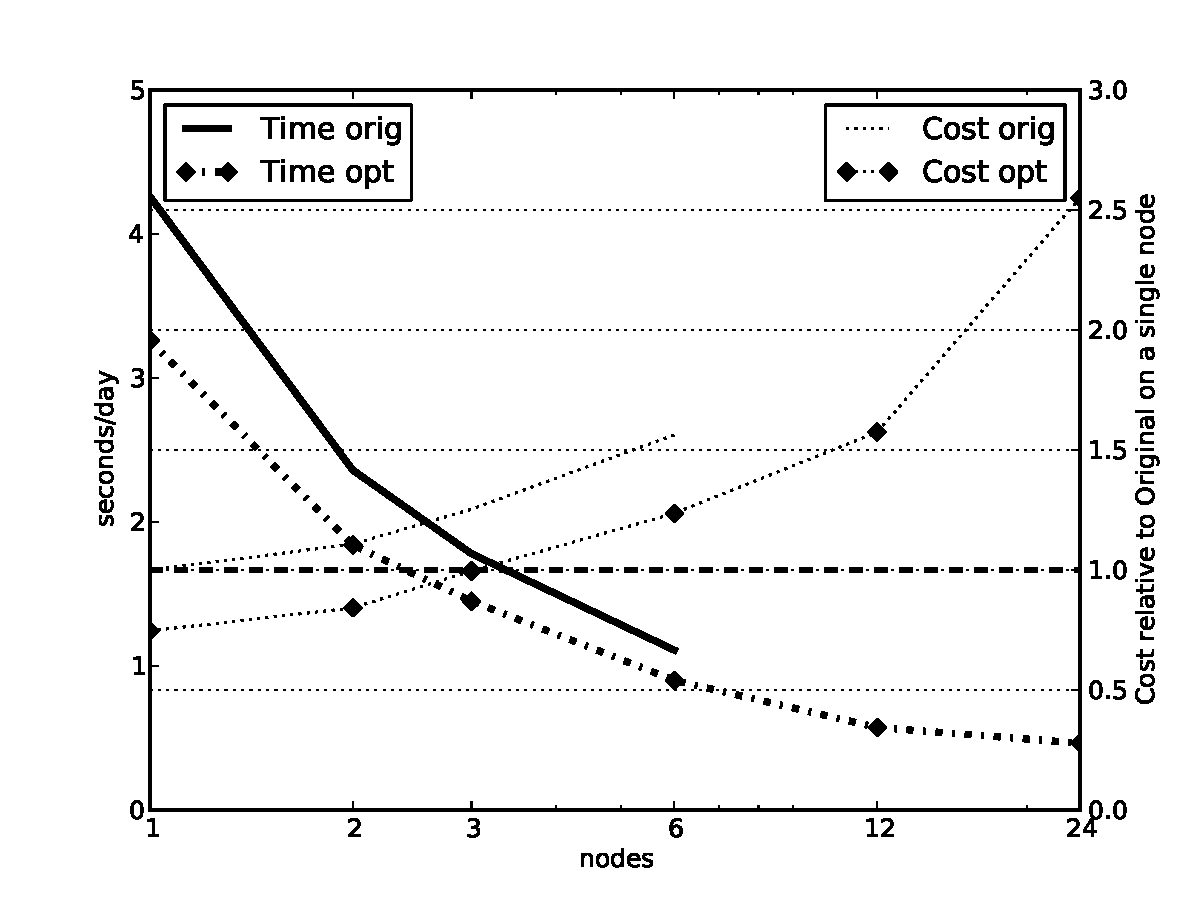
\includegraphics[width=12.0cm]{figures/homme-ys-ne4-cam.pdf}
\end{center}
\caption{Strong scaling for HOMME in perfTest configuration (ne=4, plev=26, and qsize=25)  on 1-24 nodes of Yellowstone. }
\label{fig:homme-ys-ne4}
\end{figure}

The solid blue line (labeled orig) corresponds to the version of the SE dynamical core used in CESM1, while the solid red line (labeled opt) corresponds to the version of the SE dynamical core used in CESM2.  A significant reduction in execution time for the dynamical core is apparent for both the CAM-like and WACCM-like configuration.  It is also important to note that good speedup is even achieved on problem sizes with less than a single spectral element per core. The ability to efficiently run the SE dynamical core on problem sizes that are smaller than a single spectral element per core is absolutely critical to being able to successfully utilize the increasing on-node parallelism that Xeon Phi offers.  We have also included dotted blue and red lines which indicate the cost of the dynamical core relative to the CESM1 version using 6 spectral elements per hardware core.  These cost lines allow for an easy comparison of the impact that these optimizations may have on science objectives.  Recall that our current Mira jobs have a maximum of 3 elements per hardware core.  If we draw a horizontal line from the cost to perform the CESM1 version of the SE dynamical core in the CAM-like configuration (left figure) using 3 elements per hardware core, it is apparent that we can utilize ~3 times the amount of hardware cores with only a very modest increase in computational cost using the new SE dynamical core.  Specifically, instead of using 3 elements per hardware core we can scale to 1 element per hardware core.  A similar analysis for WACCM-like configuration reveals that instead of being limited to 3 elements per hardware core, we will be able to scale to ¼ element per hardware core, enabling the use of 12 times the number of hardware cores. 



\begin{figure}[]
 \begin{center}
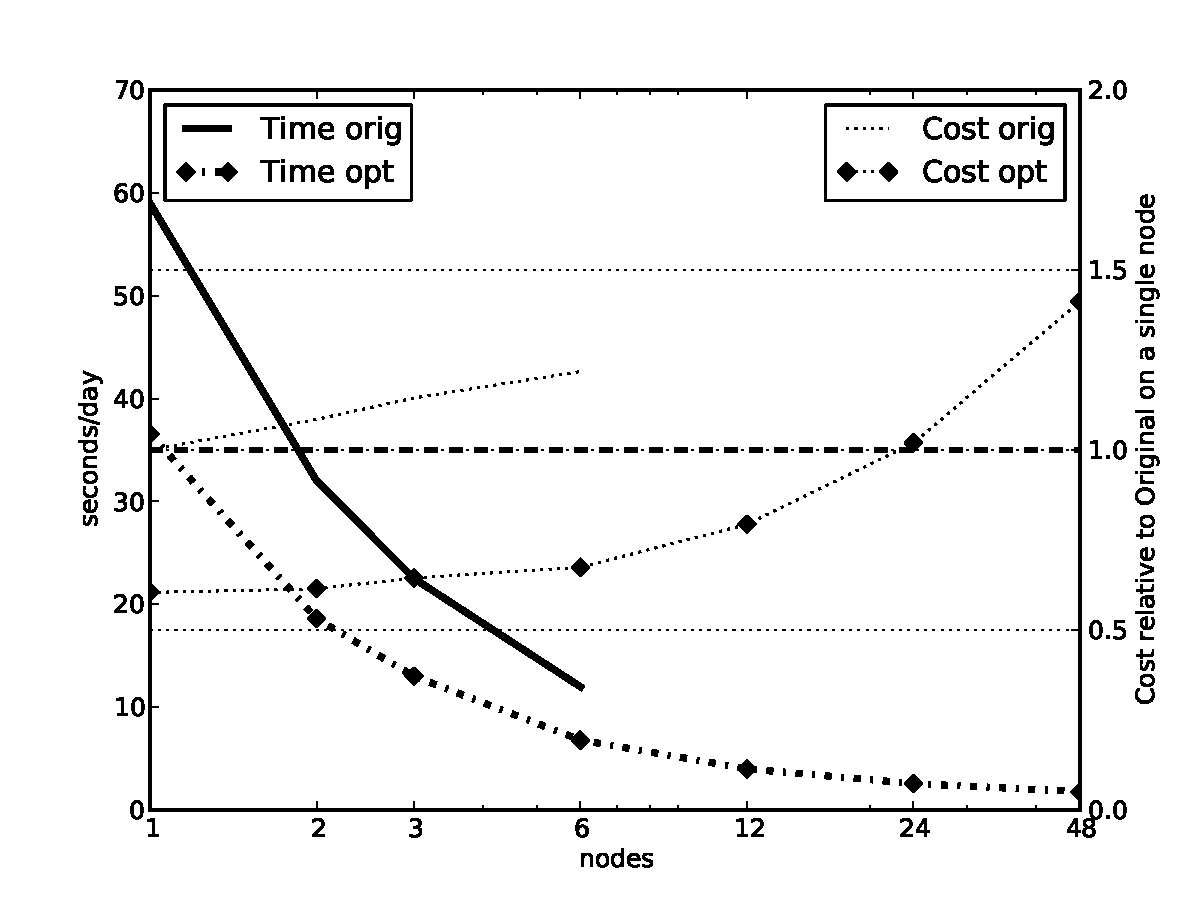
\includegraphics[width=12.0cm]{figures/homme-ys-ne4-waccm.pdf}
\end{center}
\caption{Strong scaling for HOMME in perfTestWACCM configuration (ne=4, plev=70, qsize=135) on 1-48 nodes of yellowstone.}
\label{fig:homme-ys-ne4}
\end{figure}



\begin{figure}[]
 \begin{center}
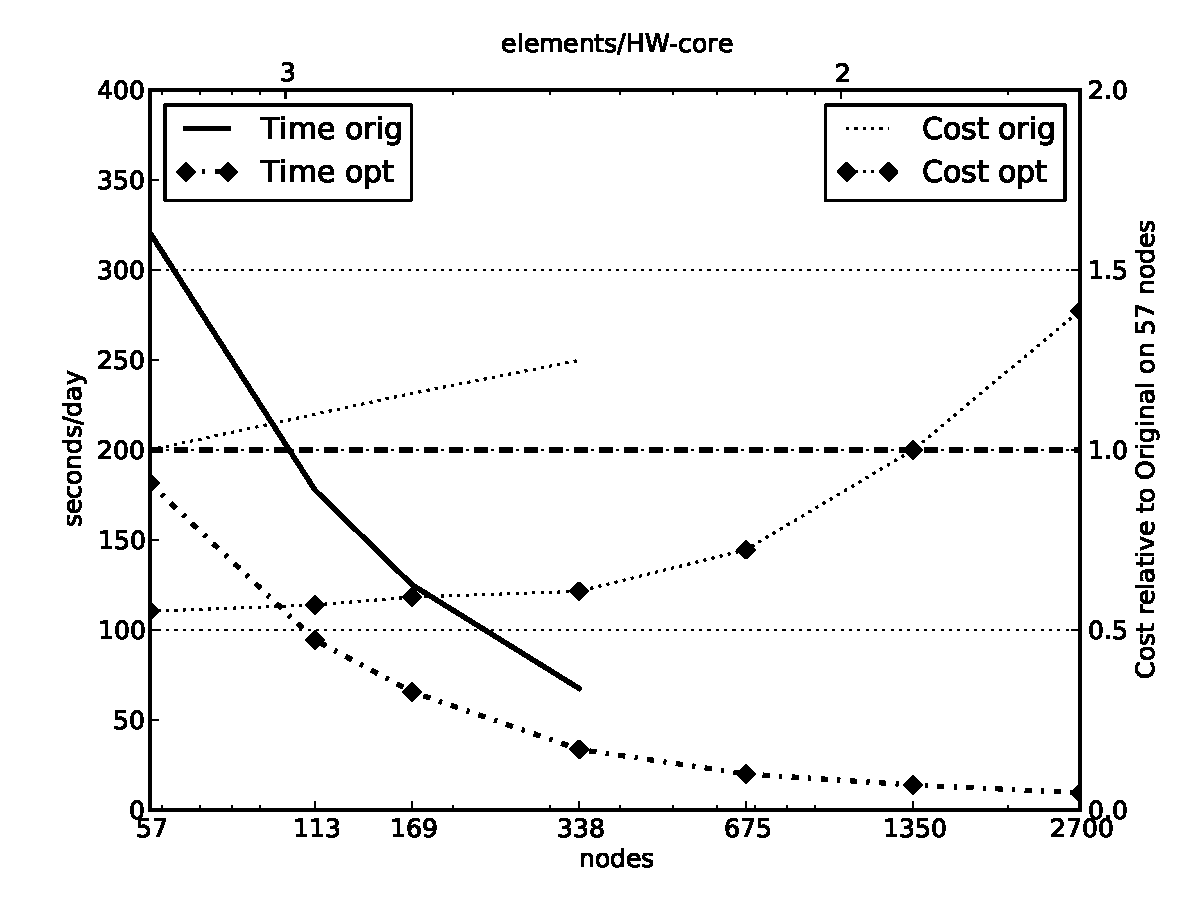
\includegraphics[width=12.0cm]{figures/homme-ys-ne30-waccm.pdf}
\end{center}
\caption{Strong scaling for HOMME in perfTestWACCM configuration (NE=30, PLEV=70, qsize=135) on 57-2700 nodes of yellowstone.{\color{red} Need extra data points for larger core counts.}}
\label{fig:homme-ys-ne30}
\end{figure}

q
Because of our IPCC-WACS project we have gained early access to single nodes of Knights Landing (KNL) hardware we are also able to provide timing results of the original and optimized SE dynamical core.  Note that when run outside of CAM the dynamical core is also known as High Order Methods Modeling Environment or HOMME.  Using this 68-core single socket system, we have been able to compare the performance of HOME on both the CAM-like and WACCM-like configurations to other single node systems.  Note that for this comparison we configure HOMME to use 384 spectral elements. We choose a larger HOMME configuration for this comparison to avoid the load-balance issues that the small configuration would create on the KNL node.  Figure 6 contains the timing for the CAM-like and WACCM-like configurations on the left and right side respectively. Results are provided for the following nodes:  a 16-core Sandybridge (SNB2), a 32-core Haswell, (HSW2), and a 68-core KNL node.  Note that in the case of the KNL node only 64 of the 68 cores are used.  It is interesting to note that while the HSW2 node is still faster than the KNL node for the CAM-like configuration, the KNL node is significantly faster for the WACCM-like configuration. We suspect that this is the result of the on-package high-bandwidth memory that KNL provides.

\begin{figure}[]
 \begin{center}
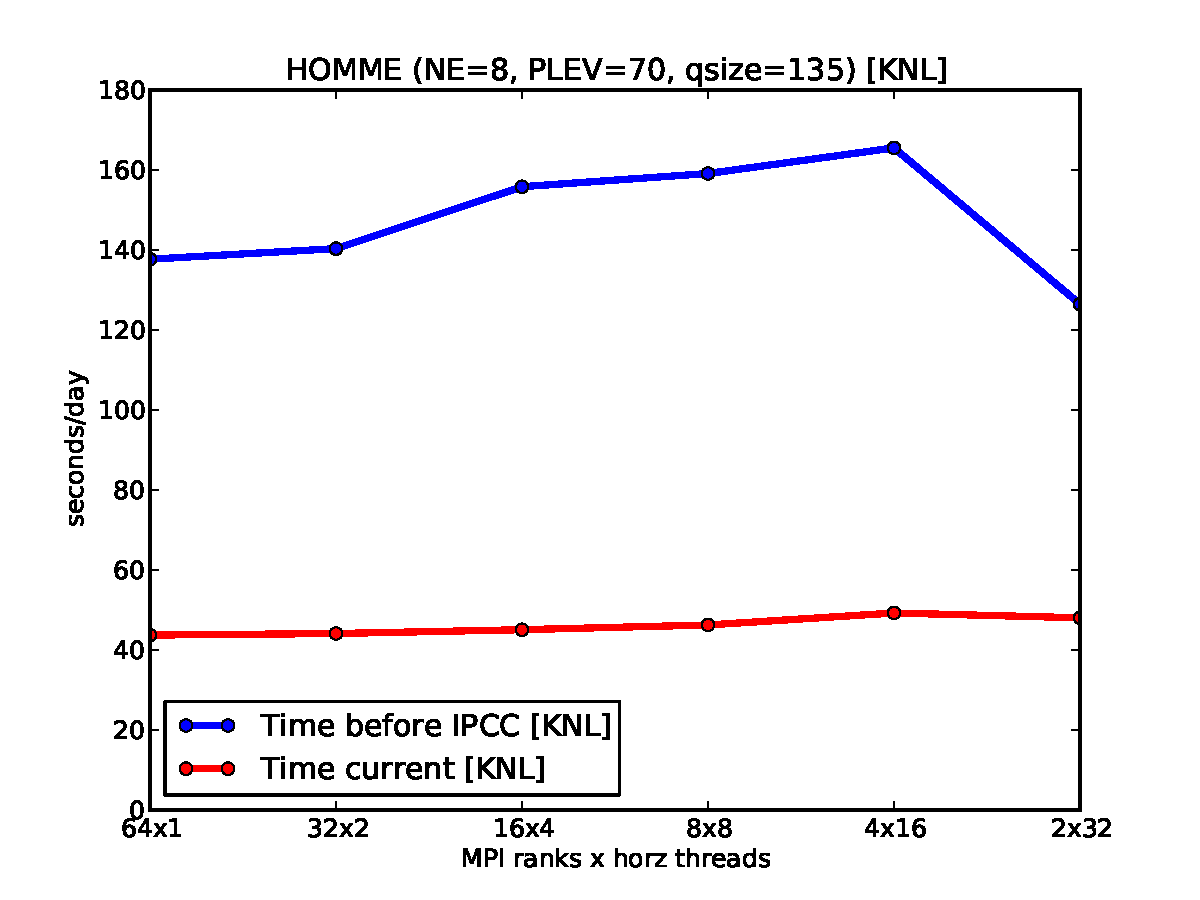
\includegraphics[width=12.0cm]{figures/homme-knl-waccm.pdf}
\end{center}
\caption{Execution time for HOMME in perfTestWACCm configuration on a single node of Knights Landing.{\color{red} Redo with updated version of HOMME.  Color is not allowed in book.  Replace line graphs with bar graphs.}}
\label{fig:homme-knl}
\end{figure}


We believe that the combined impact of both the scalability improvements within the SE dynamical core and the improved architectural features that a Knights Landing or Knights Hill based system offers will enable CESM2 to efficiently utilize 172,800 hardware cores for a single CESM ensemble member. 

